\begin{figure}[htpb]
    \centering
    \begin{subfigure}{0.49\linewidth}
        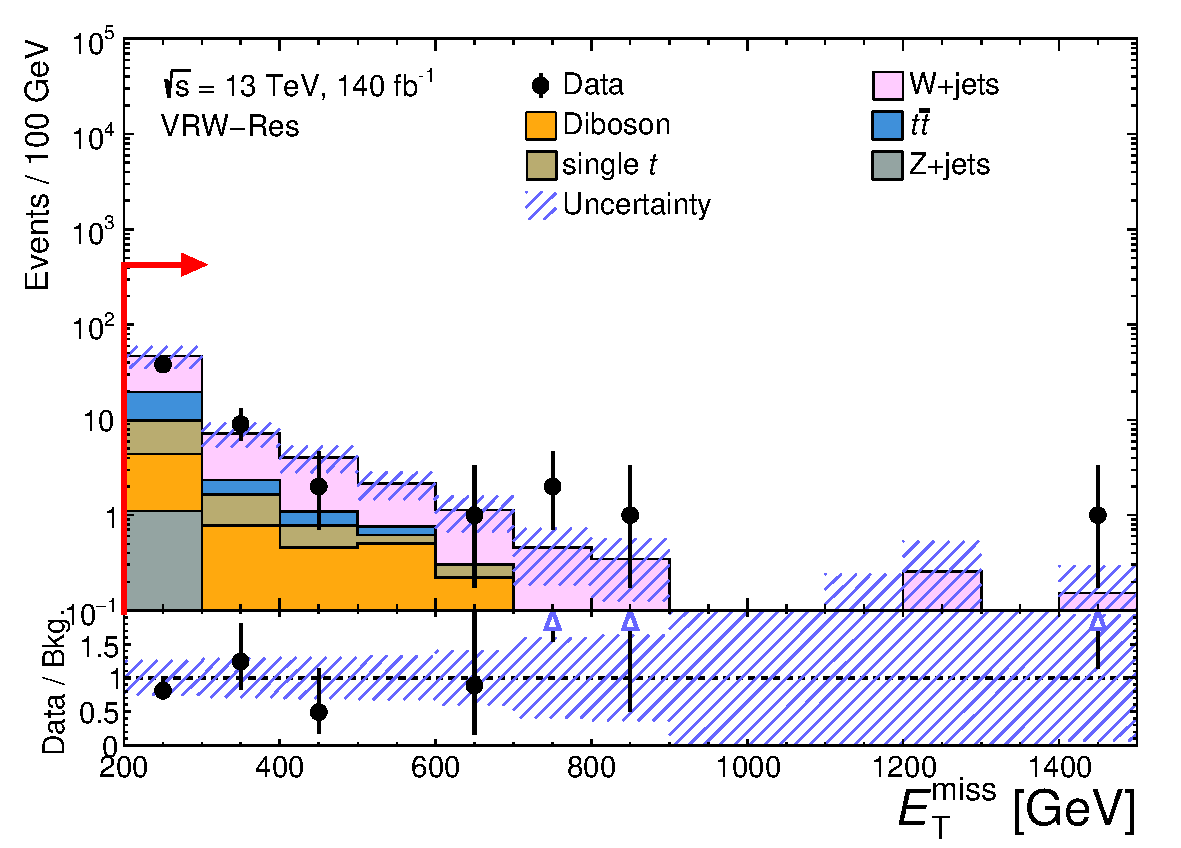
\includegraphics[width=\linewidth]{Figs/CH8/bonly/VR_0tau1l1b_Res_met_N_minus_1_met.pdf}
        \caption[]{$\met$.}
    \end{subfigure}\hfill
    \begin{subfigure}{0.49\linewidth}
        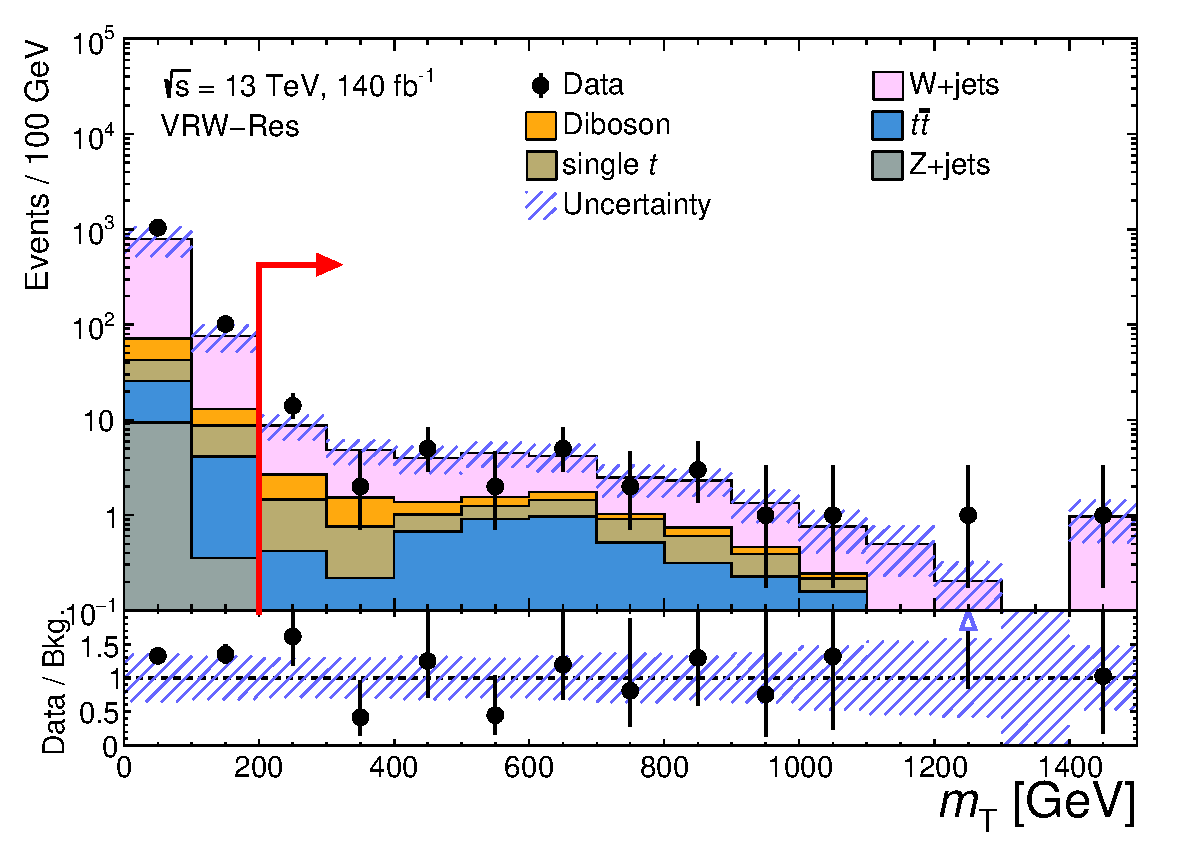
\includegraphics[width=\linewidth]{Figs/CH8/bonly/VR_0tau1l1b_Res_mT_N_minus_1_mT.pdf}
        \caption[]{$\mT^\ell$.}
    \end{subfigure}\\
    \begin{subfigure}{0.49\linewidth}
        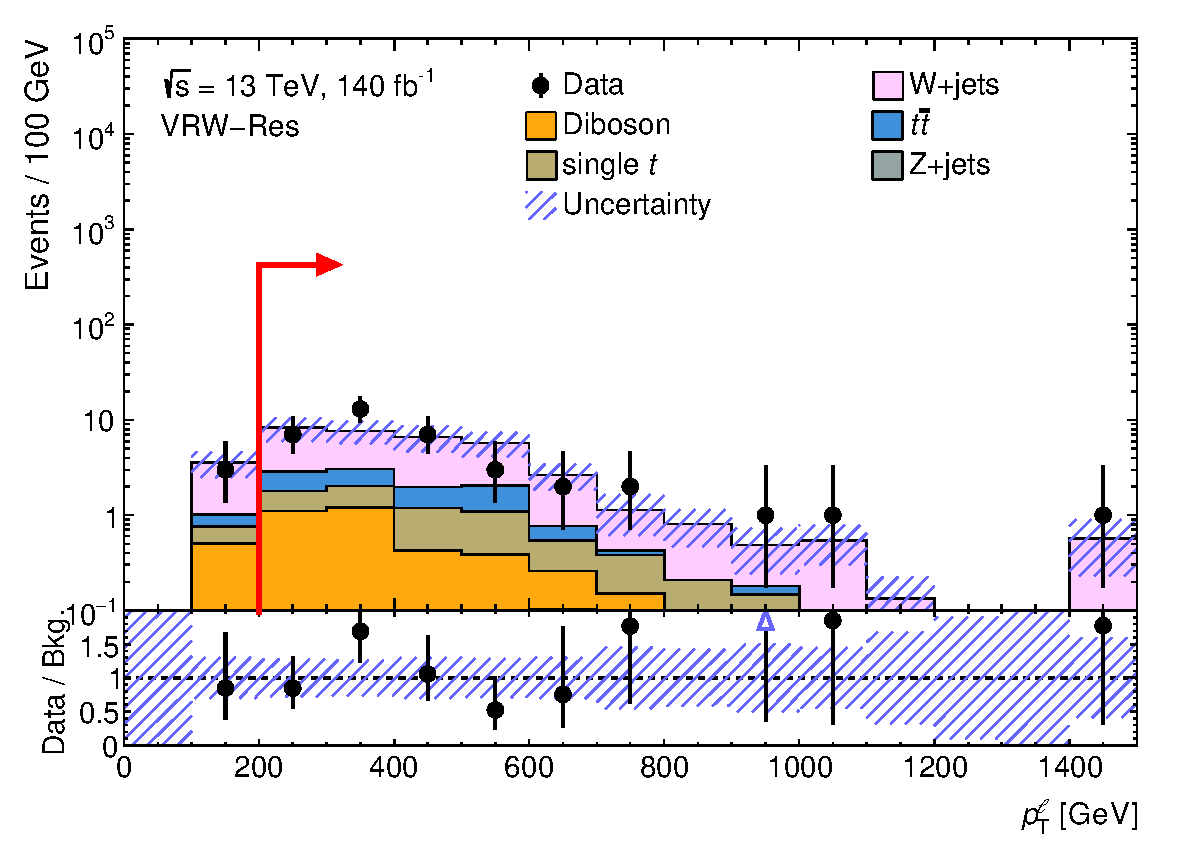
\includegraphics[width=\linewidth]{Figs/CH8/bonly/VR_0tau1l1b_Res_lep_pt_N_minus_1_lep_pt_0.pdf}
        \caption[]{$\pT^\ell$.}
    \end{subfigure}\hfill
    \begin{subfigure}{0.49\linewidth}
        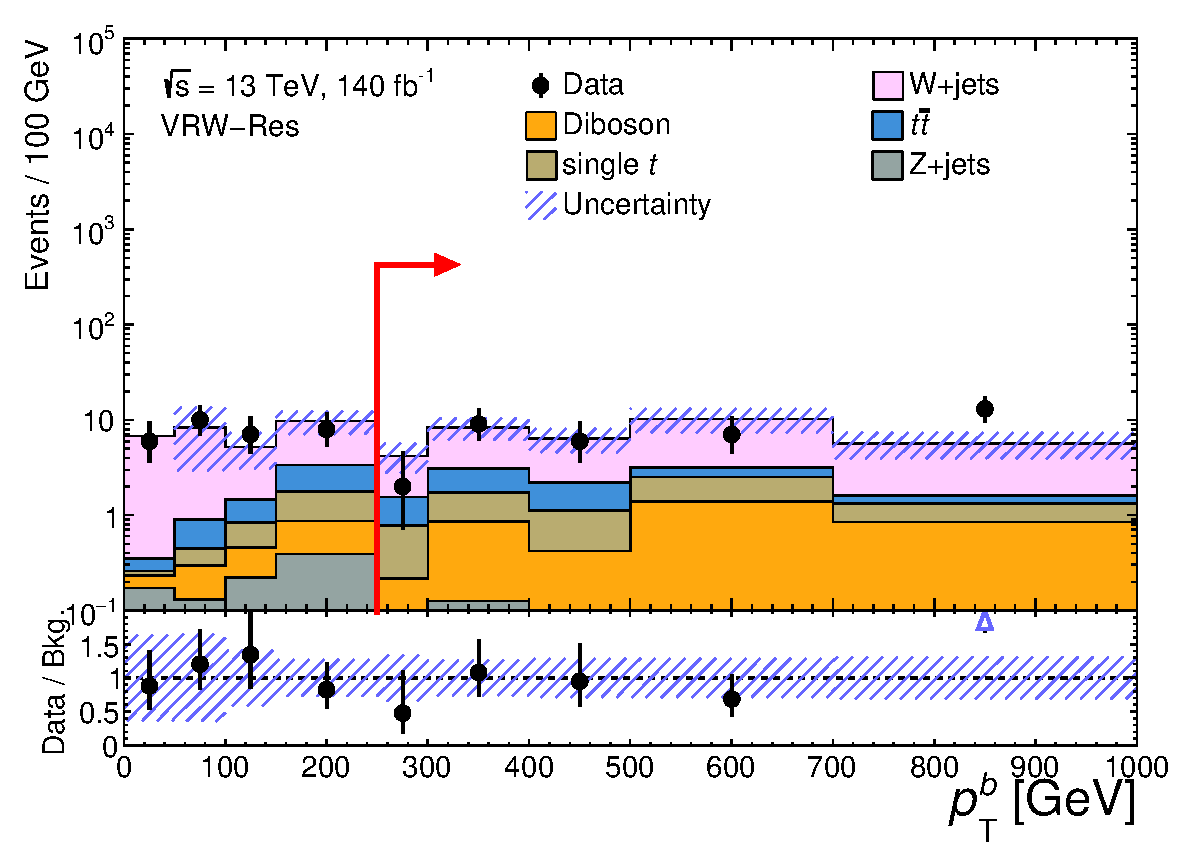
\includegraphics[width=\linewidth]{Figs/CH8/bonly/VR_0tau1l1b_Res_bjet_pt_N_minus_1_bjet_pt_0.pdf}
        \caption[]{$\pT^b$.}
    \end{subfigure}\\
    \begin{subfigure}{0.49\linewidth}
        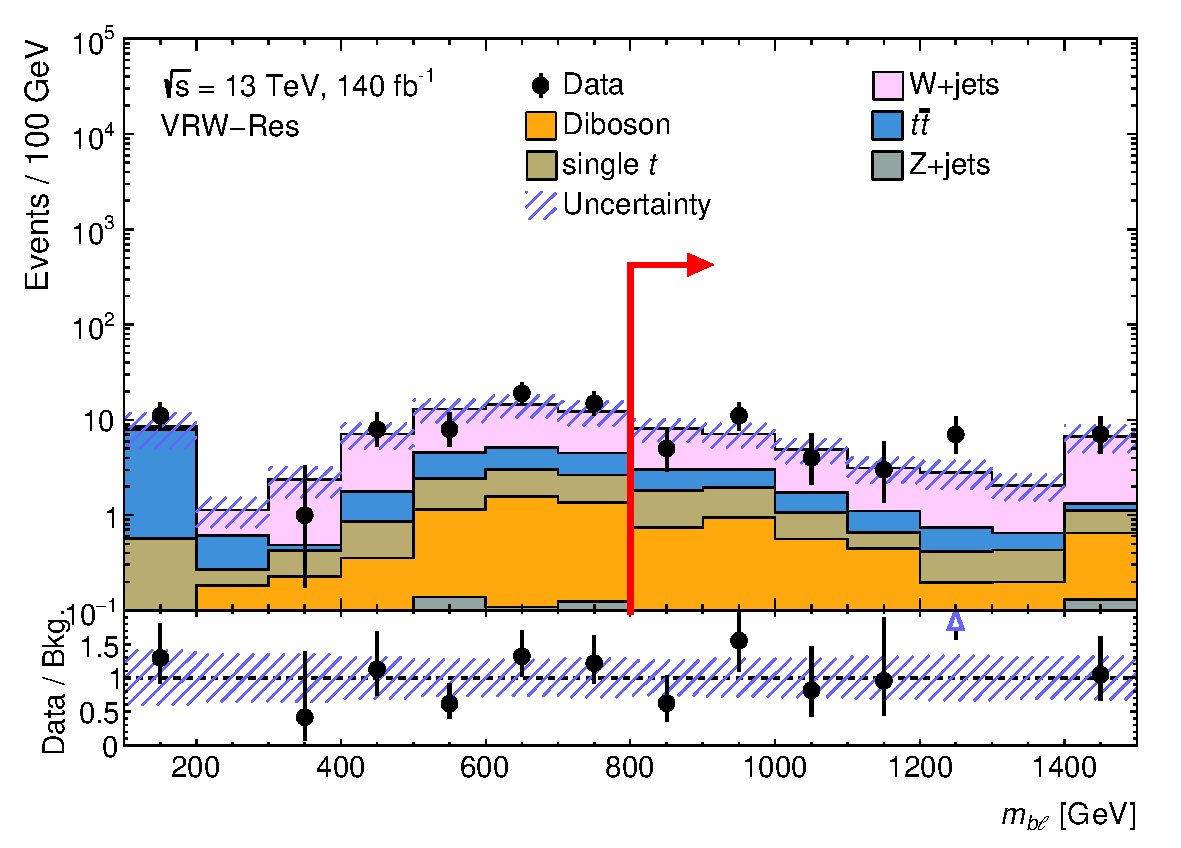
\includegraphics[width=\linewidth]{Figs/CH8/bonly/VR_0tau1l1b_Res_InvM_N_minus_1_Mlb.pdf}
        \caption[]{$m_{b\ell}$.}
    \end{subfigure}\hfill
    \begin{subfigure}{0.49\linewidth}
        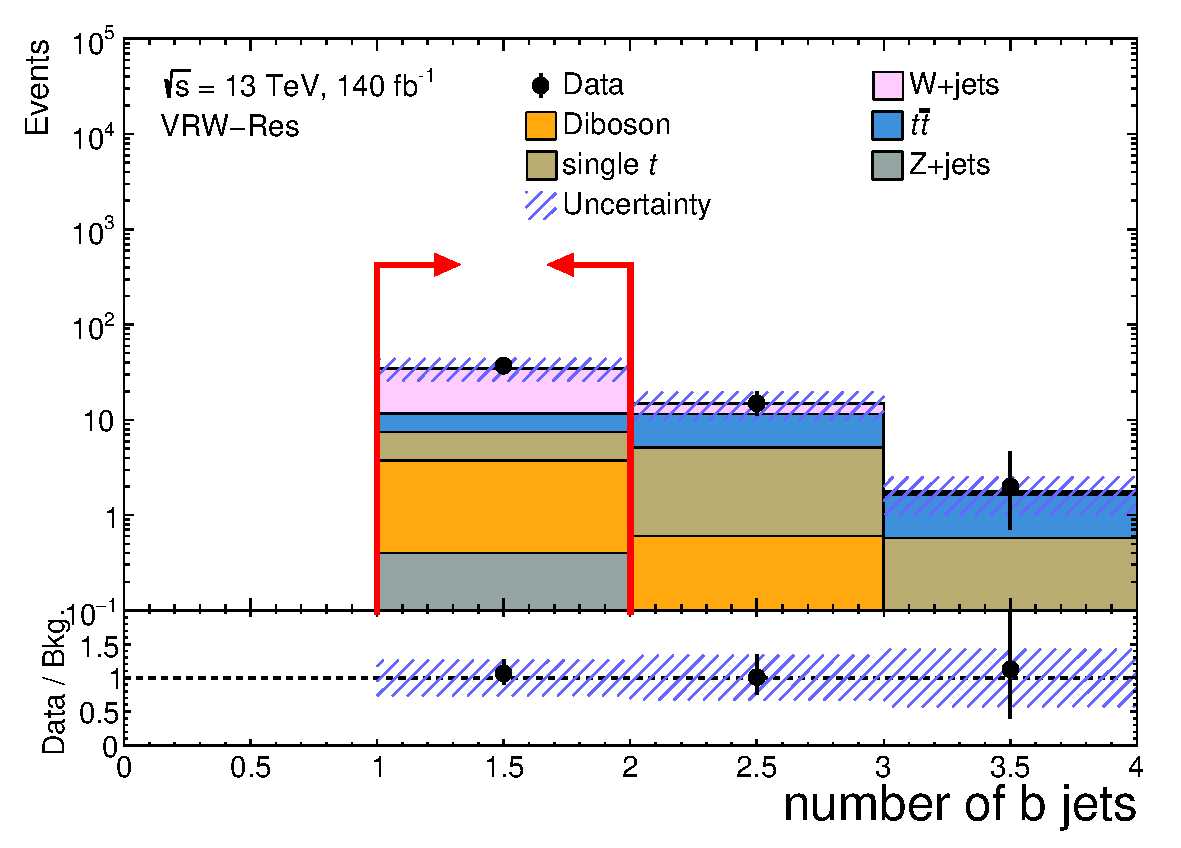
\includegraphics[width=\linewidth]{Figs/CH8/bonly/VR_0tau1l1b_Res_n_bjets_N_minus_1_n_bjets.pdf}
        \caption[]{$N_b$.}
    \end{subfigure}
    \caption[Background-only fit distributions in VRW-Res]{$N-1$ distributions in $\VRW$-$\Res$ for the combined $e$ and $\mu$ channels, after the background-only fit in CRs. The hatched bands show the combined statistical and systematic uncertainties. The bottom panels show the ratio of data to background prediction. Red arrows indicate variable thresholds for the $\VRW$ regions. The last bin includes overflow.}
    \label{fig:ch8_vrw_res}
\end{figure}

\begin{figure}[htpb]
    \centering
    \begin{subfigure}{0.49\linewidth}
        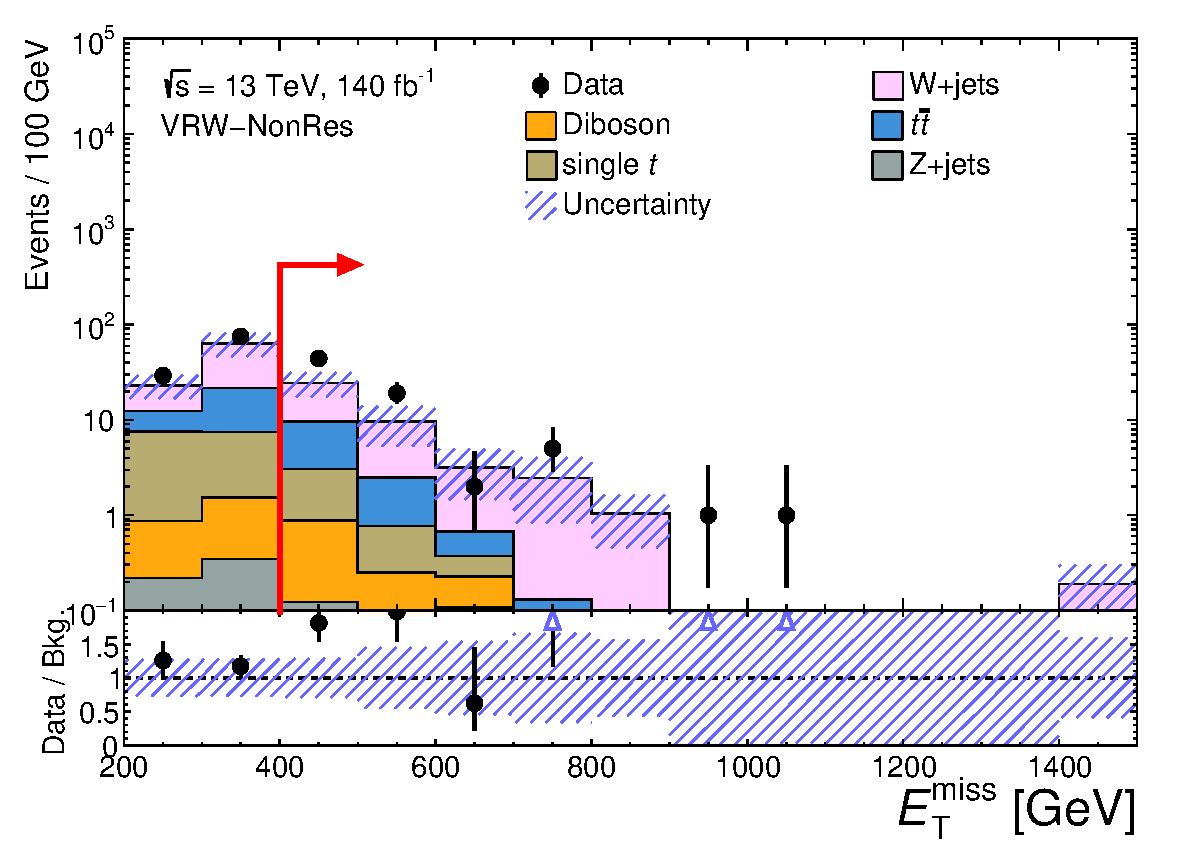
\includegraphics[width=\linewidth]{Figs/CH8/bonly/VR_0tau1l1b_NonRes_met_N_minus_1_met.pdf}
        \caption[]{$\met$.}
    \end{subfigure}\hfill
    \begin{subfigure}{0.49\linewidth}
        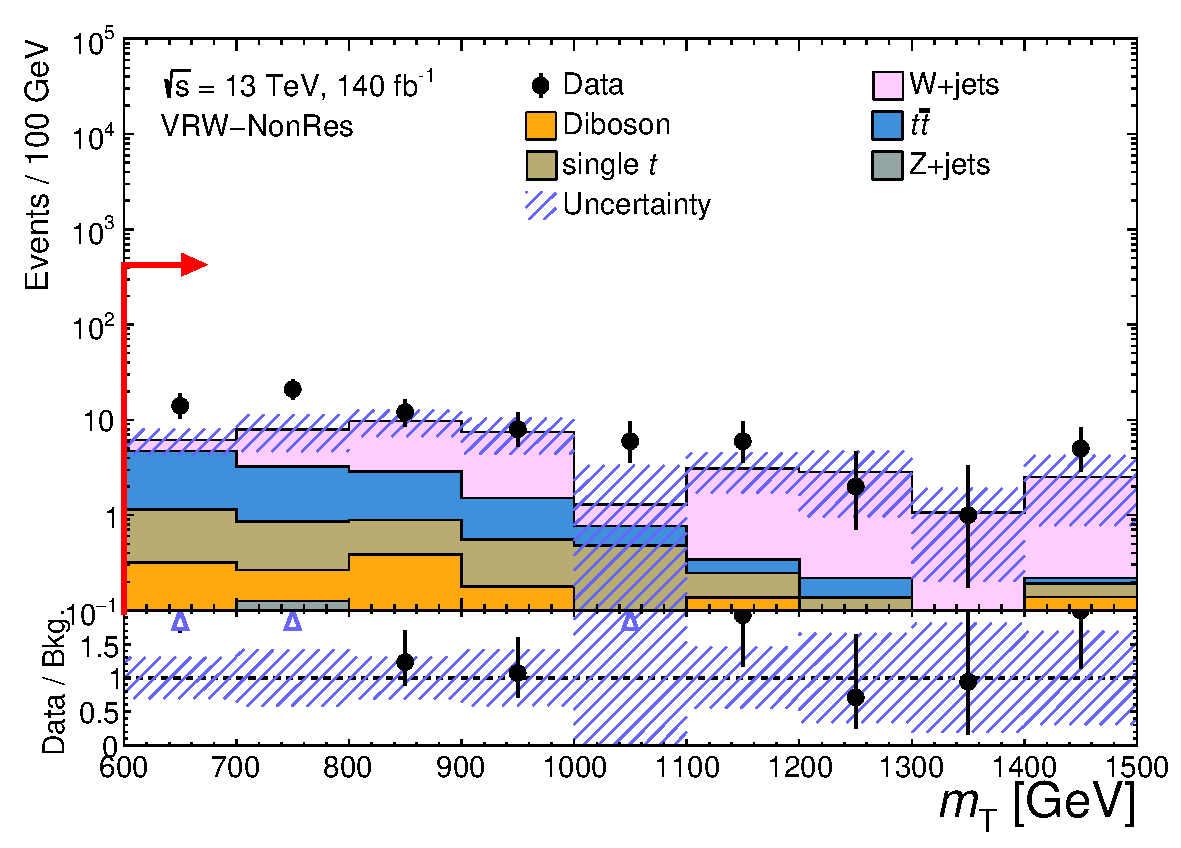
\includegraphics[width=\linewidth]{Figs/CH8/bonly/VR_0tau1l1b_NonRes_mT_N_minus_1_mT.pdf}
        \caption[]{$\mT^\ell$.}
    \end{subfigure}\\
    \begin{subfigure}{0.49\linewidth}
        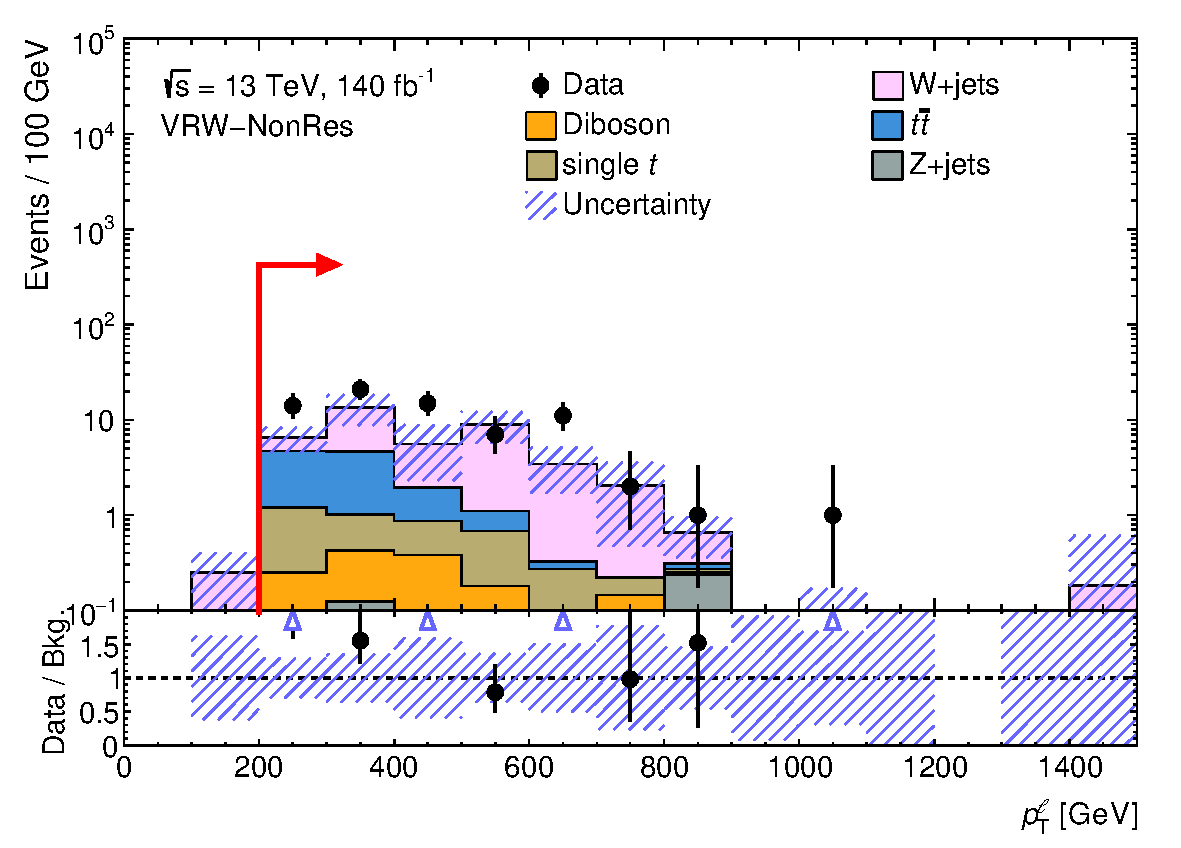
\includegraphics[width=\linewidth]{Figs/CH8/bonly/VR_0tau1l1b_NonRes_lep_pt_N_minus_1_lep_pt_0.pdf}
        \caption[]{$\pT^\ell$.}
    \end{subfigure}\hfill
    \begin{subfigure}{0.49\linewidth}
        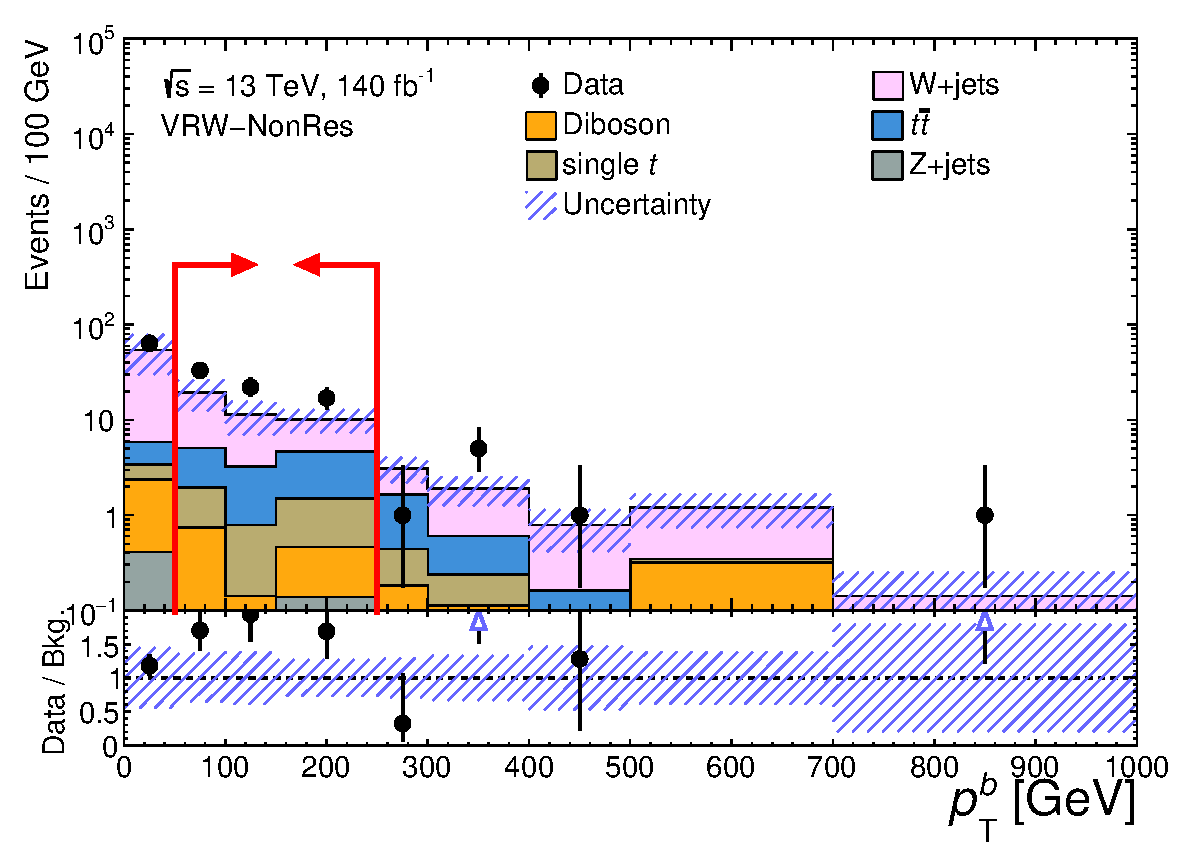
\includegraphics[width=\linewidth]{Figs/CH8/bonly/VR_0tau1l1b_NonRes_bjet_pt_N_minus_1_bjet_pt_0.pdf}
        \caption[]{$\pT^b$.}
    \end{subfigure}\\
    \begin{subfigure}{0.49\linewidth}
        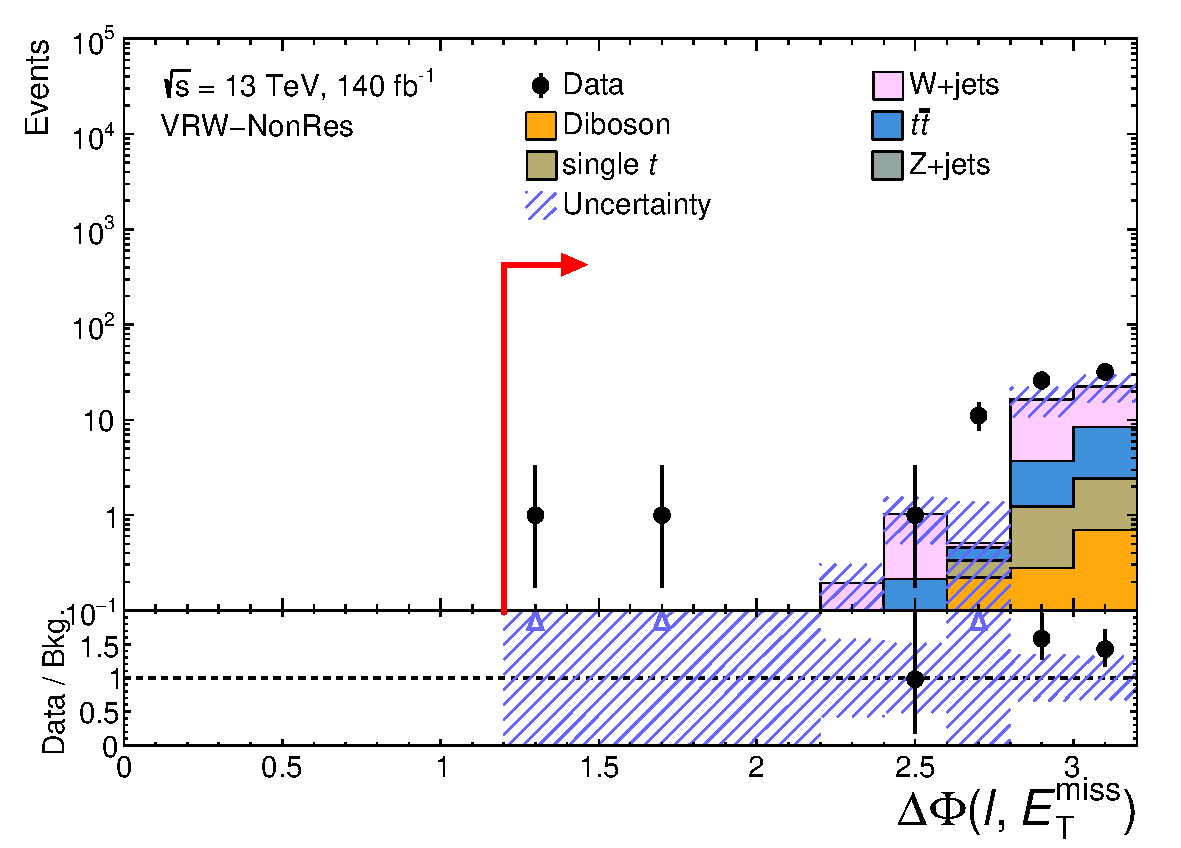
\includegraphics[width=\linewidth]{Figs/CH8/bonly/VR_0tau1l1b_NonRes_dphi_N_minus_1_dphi_lmet.pdf}
        \caption[]{$\DphiLepMet$.}
    \end{subfigure}\hfill
    \begin{subfigure}{0.49\linewidth}
        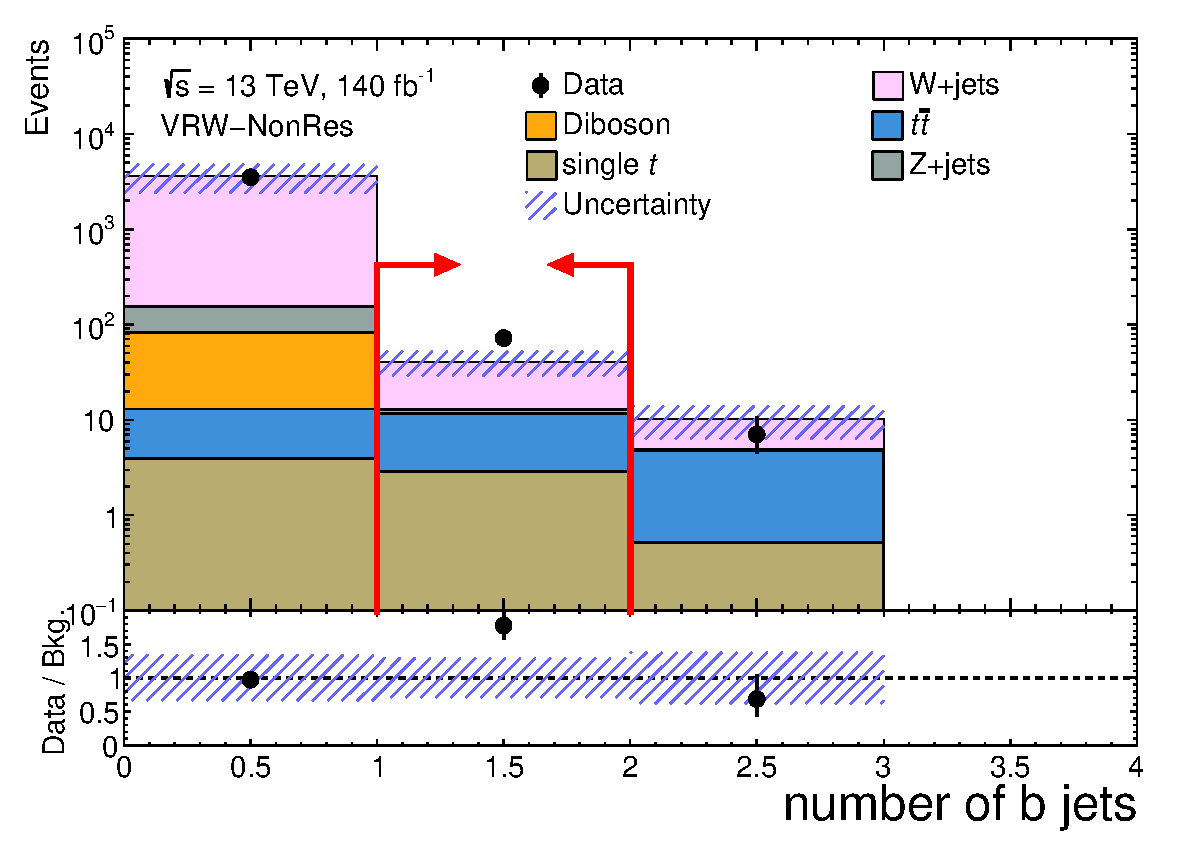
\includegraphics[width=\linewidth]{Figs/CH8/bonly/VR_0tau1l1b_NonRes_n_bjets_N_minus_1_n_bjets.pdf}
        \caption[]{$N_b$.}
    \end{subfigure}
    \caption[Background-only fit distributions in VRW-NonRes]{$N-1$ distributions in $\VRW$-$\NonRes$ for the combined $e$ and $\mu$ channels, after the background-only fit in CRs. The hatched bands show the combined statistical and systematic uncertainties. The bottom panels show the ratio of data to background prediction. Red arrows indicate variable thresholds for the $\VRW$ regions. The last bin includes overflow.}
    \label{fig:ch8_vrw_nonres}
\end{figure}
